%\documentclass[11pt]{article}
%\usepackage[top=1.5cm,bottom=2cm,left=2cm,right= 2cm]{geometry}
%\geometry{letterpaper}                   % ... or a4paper or a5paper or ... 
%%\geometry{landscape}                % Activate for for rotated page geometry
%\usepackage[parfill]{parskip}    % Activate to begin paragraphs with an empty line rather than an indent
%\usepackage{amssymb}
%\usepackage{epstopdf}
%\usepackage{amsmath}            
%\usepackage{multirow}    
%\usepackage{multicol}    
%\usepackage{changepage}
%\usepackage{lscape}
%\usepackage{enumerate}
%\usepackage{ulem}
%\DeclareGraphicsRule{.tif}{png}{.png}{`convert #1 `dirname #1`/`basename #1 .tif`.png}
%
%\usepackage{xcolor}
%
%\usepackage[colorlinks=false,pdfborder={0 0 0},urlcolor= dark,colorlinks=true,linkcolor=black]{hyperref}
%
%\definecolor{custom_blue}{rgb}{.337,.608,.741}
%
%\newcommand{\note}[1]{\textcolor{red}{\textbf{{#1}}}}
%\newcommand{\urlwofont}[1]{\urlstyle{same}{\url{#1}}}
%
%\renewcommand{\emph}[1]{\textit{#1}}
%
%%\date{}                                           % Activate to display a given date or no date

\documentclass[11pt]{article}

%%%%%%%%%%%%%%%%
% Packages
%%%%%%%%%%%%%%%%

\usepackage[top=2cm,bottom=2cm,left=1.5cm,right= 1.5cm]{geometry}
\usepackage[parfill]{parskip}
\usepackage{graphicx, xcolor,multicol, enumerate, setspace, changepage, amsmath, enumerate, amssymb}
\DeclareGraphicsRule{.tif}{png}{.png}{`convert #1 `dirname #1`/`basename #1 .tif`.png}


%%%%%%%%%%%%%%%%
% User defined colors
%%%%%%%%%%%%%%%%

% Pantone 2015 Spring colors
% http://iwork3.us/2014/09/16/pantone-2015-spring-fashion-report/
% update each semester or year

\xdefinecolor{custom_blue}{rgb}{0, 0.70, 0.79} % scuba blue
\xdefinecolor{custom_darkBlue}{rgb}{0.11, 0.31, 0.54} % classic blue
\xdefinecolor{custom_orange}{rgb}{0.97, 0.57, 0.34} % tangerine
\xdefinecolor{custom_green}{rgb}{0.49, 0.81, 0.71} % lucite green
\xdefinecolor{custom_red}{rgb}{0.58, 0.32, 0.32} % marsala

\xdefinecolor{custom_lightGray}{rgb}{0.78, 0.80, 0.80} % glacier gray
\xdefinecolor{custom_darkGray}{rgb}{0.54, 0.52, 0.53} % titanium


%%%%%%%%%%%%%%%%
% From OI
%%%%%%%%%%%%%%%%

% expected counts
\newcommand{\ec}[1]{\textcolor{custom_blue}{\footnotesize{~(#1)}}}

% parts environment
\newenvironment{parts}{
\vspace{-0.25cm}
\begin{enumerate}[(a)]
\setlength{\itemsep}{0mm}
}
{\end{enumerate}
}

% subparts environment
\newenvironment{subparts}{
\begin{enumerate}[i.]
\setlength{\itemsep}{0mm}
}
{\end{enumerate}
}

% romanparts environment
\newenvironment{romanparts}{
\begin{enumerate}[I.]
\setlength{\itemsep}{0mm}
}
{\end{enumerate}
}

% hypotheses environment
\newenvironment{hyp}{
\begin{itemize}
\setlength{\itemsep}{0mm}
}
{\end{itemize}
}

% conditions environment
\newenvironment{cond}{
\begin{enumerate}[1.]
\setlength{\itemsep}{0mm}
}
{\end{enumerate}
}

%%%%%%%%%%%%%%%%
% Begin document
%%%%%%%%%%%%%%%%

\begin{document}

$\:$ \\
\vspace{2cm}

{\LARGE \textcolor{custom_blue}{\textbf{Practice problems - Midterm 1}}}

The midterm will cover everything we have covered so far in Units 1 - 3.

When studying for the exam you should review the assigned and practice homework questions you've had so far as well as any other questions from the book in the sections we've covered. I've selected a sample of problems from each chapter and included worked out solutions below. You shouldn't limit your studying to just these problems, but these might be good to have the detailed answers for. Work on the problems on your own first, then check your answers against the key starting on the next page.

\begin{itemize}
\renewcommand\labelitemi{\textcolor{custom_blue}{{\footnotesize $\blacksquare$}}}
\item Chp 1: 19, 41, 51, 53
\item Chp 2: 3, 7, 17, 25
\item Chp 3: 5, 11, 27, 31
\item Chp 4: 7, 23, 27, 41, 43, 45%, 47, 49
\end{itemize}



\pagebreak

{\Large \textcolor{custom_blue}{\textbf{Chapter 1}}}

\begin{enumerate}

\item[1.19] 
\begin{parts}
\item Experiment, since the researchers randomly assigned different treatments to the participants.
\item Response variable: Duration of the cold. \\
Explanatory variable: Treatment, with 4 levels; placebo, 1g, 3g, 3g with additives.
\item The patients were blinded as they did not know which treatment they received.
\item The study was double-blind with respect to the researchers evaluating the patients, but the nurses who briefly interacted with patients during the distribution of the medication were not blinded. (It was partially double-blind.)
\item Since the patients were randomly assigned to the treatment groups and they are blinded we would expect about an equal number of patients in each group to not adhere to the treatment. While this means that final results of the study will be based on fewer number of participants, non-adherence does not introduce a confounding variable to the study. 
\end{parts}

\item[1.41]
\begin{parts}
\item The median is a much better measure of the typical amount earned by these 42 people. The mean is much higher than the income of 40 of the 42 people. This is because the mean is an arithmetic average and gets affected by the two extreme observations. The median does not get effected as much since it is robust to outliers.
\item The IQR  is a much better measure of variability in the amounts earned by nearly all of the 42 people. The standard deviation gets affected greatly by the two high salaries, but the IQR is robust to these extreme observations.
\end{parts}

\item[1.51]
\begin{parts}
\item False. Instead of comparing counts, we should compare percentages of people in each group who suffered cardiovascular problems.
\item True.
\item False. Association does not imply causation. We cannot infer a causal relationship based on an observational study. (We cannot say changing the drug a person is on affects her risk, which is why part (b) is true. The difference in these statements is subtle.)
\item True.
\end{parts}

\item[1.53]
\begin{parts}
\item Proportion of all patients who had a heart attack: $\frac{7,979}{227,571} \approx 0.035$
\item Expected number of heart attacks in the rosiglitazone group if having cardiovascular problems and treatment were independent can be calculated as the number of patients in that group multiplied by the overall cardiovascular problem rate in the study: $67,593 * \frac{7,979}{227,571} \approx 2370$.
\item 
\begin{subparts}
\item $H_0$: Independence model. The treatment and cardiovascular problems are independent. They have no relationship, and the difference in incidence rates between the rosiglitazone and pioglitazone groups is due to chance.
$H_A$: Alternate model. The treatment and cardiovascular problems are not independent. The difference in the incidence rates between the rosiglitazone and pioglitazone groups is not due to chance and rosiglitazone is associated with an increased risk of serious cardiovascular problems.
\item A higher number of patients with cardiovascular problems than expected under the assumption of independence would provide support for the alternative hypothesis as this would suggest that rosiglitazone increases the risk of such problems.
\item In the actual study, we observed 2,593 cardiovascular events in the rosiglitazone group. In the 1,000 simulations under the independence model, we observed somewhat less than 2,593 in every single simulation, which suggests that the actual results did not come from the independence model. That is, the variables do not appear to be independent, and we reject the independence model in favor of the alternative. The study's results provide convincing evidence that rosiglitazone is associated with an increased risk of cardiovascular problems.
\end{subparts}
\end{parts}

\end{enumerate}

%

{\Large \textcolor{custom_blue}{\textbf{Chapter 2}}}

\begin{enumerate}
\item[2.3]
\begin{parts}
\item 10 tosses. Since the desired outcome is larger than the expected proportion of heads (50\%), we would want fewer trials (flips). With a low number of flips the variability in the number of heads observed is much larger. For example, we wouldn't be very surprised if 7 out of 10 flips were heads. On the other hand, with 100 flips, we would often be surprised if 70 out of 100 flips were heads. With 100 flips it would often be more likely to get something very close to 50\% heads and 50\% tails, which is not what we want.
\item 100 tosses. The expected proportion of 50\% is greater than 40\%, and with more flips the observed proportion of heads would often be closer to the expected value than if we used a sample size of 10.
\item 100 tosses. The expected proportion of 50\% is between 40\% and 60\%. With more flips the observed proportion of heads would often be closer to the expected value than if we used a sample size of 10.
\item 10 tosses. The desired proportion of heads (less than 30\%) is below the expected proportion, and with fewer flips it would often be more likely to observe a proportion that is not close to the expected value.
\end{parts}

\item[2.7] 
\begin{parts}
\item No, there are voters who are both independent and swing voters.
\item The Venn diagram is shown below.
  \begin{center}
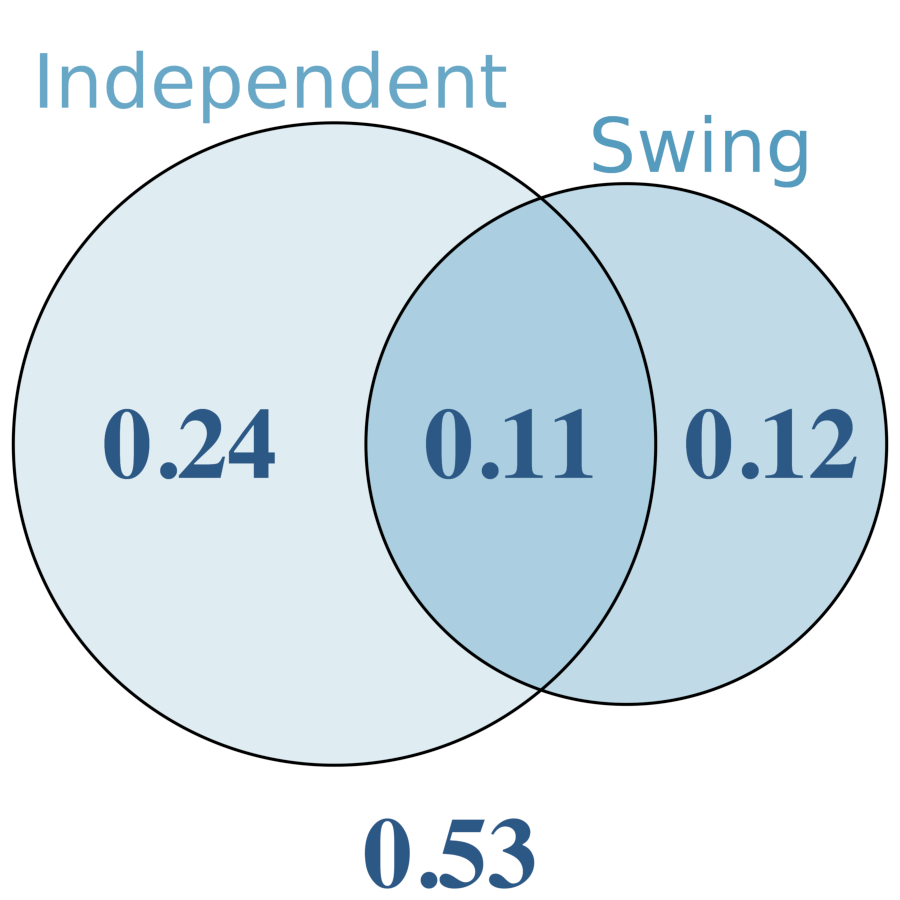
\includegraphics[width=0.2\textwidth]{figures/02/indepSwing}
  \end{center}
\item Each Independent voter is either a swing voter or not. Since 35\% of voters are Independents and 11\% are both Independent and swing voters, the other 24\% must not be swing voters.
\item Use the General Addition Rule:
\begin{align*}
P(\text{Independent or swing}) &= P(\text{Independent}) + P(\text{swing}) - P(\text{Independent and swing}) \\
&= 0.35 + 0.23 - 0.11 = 0.47
\end{align*}
\item P(neither Independent nor swing) = 1 - P(Independent or swing)  = 1 - 0.47 = 0.53.
\item P(Independent) $\times$ P(swing) = $0.35\times0.23 = 0.08$, which does not equal P(Independent and swing) = 0.11, so the events are dependent.
\end{parts}

\item[2.17]
\begin{parts}
\item P(earth is warming or liberal Democrat) = \\
= P(earth is warming) + P(liberal Democrat)  - P(earth is warming and liberal Democrat) \\
= 0.60 + 0.20 - 0.18 = 0.62
\item P(earth is warming $|$ liberal Democrat) = $\frac{0.18}{0.20} = 0.9$
\item P(earth is warming $|$ conservative Republican) = $\frac{0.11}{0.33} = 0.33$
\item No, the two appear to be dependent. The percentages of conservative Republicans and liberal Democrats who believe that there is solid evidence that the average temperature on earth has been getting warmer over the past few decades are very different.
\item P(moderate/liberal Republican $|$ not warming) = $\frac{0.06}{0.34} = 0.18$
\end{parts}

\item[2.25] $\:$ \\
\begin{center}
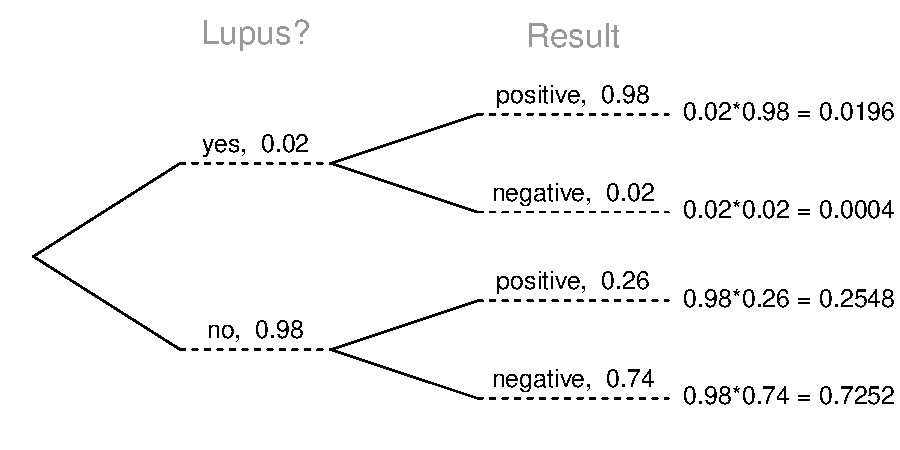
\includegraphics[width=0.6\textwidth]{figures/02/tree_lupus}
\end{center}
\[ P(lupus | positive) = \frac{P(lupus~and~positive)}{P(positive)} = \frac{0.0196}{0.0196 + 0.2548} = 0.0714 \]
Even when a patient tests positive for lupus, there is only a 7.14\% chance that he actually has lupus. House may be right.

\end{enumerate}

%

\vspace{1cm}

{\Large \textcolor{custom_blue}{\textbf{Chapter 3}}}

\begin{enumerate}
\item[3.5]
\begin{parts}
\item The Z score corresponding to the $80^{th}$ percentile of the normal distribution is approximately 0.84. Then,
\[ Z = 0.84 = \frac{y - 584}{151} \ \to\ y = 0.84 \times 151 + 584 = 710.84 \approx 711 \]
\item If a student scored worse than 70\% of the test takers, it means she scored in the $30^{th}$ percentile. The Z score corresponding to the $30^{th}$ percentile of the normal distribution is approximately -0.52. Then,
\[ Z = -0.52 = \frac{x - 462}{119} \ \to\ x = -0.52 \times 119 + 462 = 400.12 \approx 400 \]
\end{parts}

\item[3.11] 
\begin{parts}
\item The Z score corresponding to the upper 25\% of the distribution is 0.67.
\item x = 1800, $\mu$ = 1650.
\item The standard deviation of the distribution ($\sigma$) can be calculated as follows: \\
\begin{minipage}[c]{0.5 \textwidth}
\begin{align*}
Z &= \frac{x - \mu}{\sigma} \\
0.67 &= \frac{1800 - 1650}{\sigma} \\
\sigma &= \frac{1800 - 1650}{0.67} \\
\sigma &= \$ 223.88
\end{align*}
\end{minipage}
\begin{minipage}[c]{0.5\textwidth}
\begin{center}
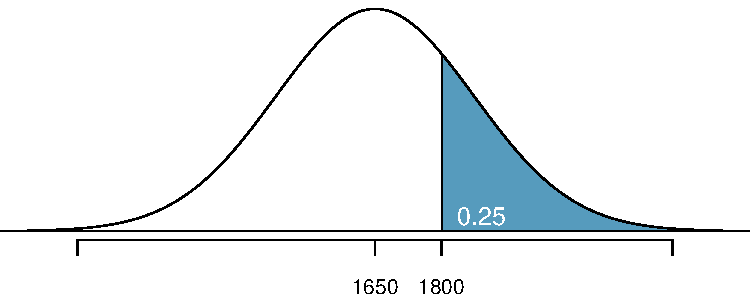
\includegraphics[width=\textwidth]{figures/03/ins_1800}
\end{center}
\end{minipage}
\end{parts}

\item[3.27]
\begin{parts}
\item In order to determine if we can we use the binomial distribution to calculate the probability of finding exactly six people out of a random sample of the ten 18-20 year olds who consumed alcoholic beverages, we need to check if the binomial conditions are met:
\begin{cond}
\item Independent trials: In a random sample, whether or not one 18-20 year old has consumed alcohol does not depend on whether or not another one has.
\item Fixed number of trials: $n = 10$.
\item Only two outcomes at each trial: Consumed or did not consume alcohol.
\item Probability of a success is the same for each trial: $p = 0.7$.
\end{cond}

\item Let X = number of people who have consumed alcohol in the group, then, using a binomial distribution with $n = 10$ and $p = 0.7$:
\[ P(X = 6) = {10 \choose 6} \times 0.7^6 \times 0.3^4 = 210 \times 0.7^6 \times 0.3^4 = 0.2 \]

\item P(6 out of 10 have consumed alcohol) = P(4 out of 10 have not consumed alcohol) = 0.2

\item P(at most 2) = P(less than or equal to 2) \\
Let $X$ be the number of people who have consumed alcohol in the group. Then, using a binomial distribution with $n = 5$ and $p = 0.7$: 
\begin{align*}
P(X \le 2) &= P(X = 0) + P(X = 1) + P(X = 2) \\
&= {5 \choose 0} \times 0.7^0 \times 0.3^5 + {5 \choose 1} \times 0.7^1 \times 0.3^4 + {5 \choose 2} \times 0.7^2 \times 0.3^3 \\
&= 0.00243 + 0.02835 + 0.1323  \\
&= 0.163
\end{align*}

\item P(at least 1) = P(greater than or equal to 1): 
\begin{align*}
P(X \ge 1) &= P(X = 1) + P(X = 2) + \cdots + P(X = 5) \\
&= 1 - P(X = 0) \\
&= 1 - 0.00243 \\
&= 0.99757
\end{align*}

\end{parts}

\item[3.31]
Let $X$ be the number of students among the 2,500 who decide to attend this university. $X$ has a binomial distribution with number of trials $n = 2,500$ and $p = 0.70$.  The university will not have enough spots if $X \ge 1787$, and we use the normal approximation to the binomial to calculate this probability. The mean and standard deviation of this distribution are
\[ \mu = np = 2,500 \times 0.7 = 1750 \qquad \sigma = \sqrt{np(1-p)} = \sqrt{2,500 \times 0.7 \times 0.3} \approx 23 \]
Then, the probability can be calculated as

\begin{minipage}[c]{0.6\textwidth}
\begin{align*}
P(X \ge 1787)  &= P \left( Z > \frac{1787 - 1750}{23} \right) \\
&= P(Z > 1.61) \\
&= 1 -  0.9463 \\
&= 0.0537
\end{align*}
\end{minipage}
\begin{minipage}[c]{0.4\textwidth}
\begin{center}
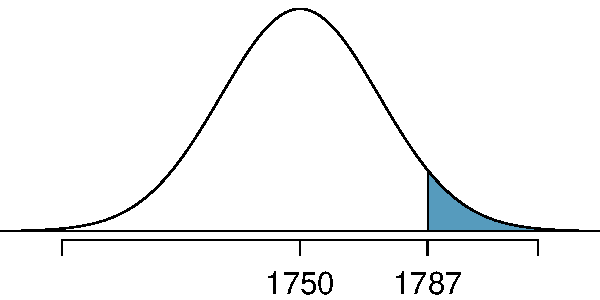
\includegraphics[width=\textwidth]{figures/03/admission_gt1787}
\end{center}
\end{minipage}

\end{enumerate}

%

\pagebreak

{\Large \textcolor{custom_blue}{\textbf{Chapter 4}}}

\begin{enumerate}
\item[4.7]
\begin{parts}
\item We are 95\% confident that that US residents spend an average of 3.53 to 3.83 hours per day relaxing or pursuing activities they enjoy after an average work day.
\item 95\% of random samples of size 1,154 will yield a confidence interval that contains the true average hours per day that US residents spend relaxing or pursuing activities they enjoy after an average work day.
\item A 90\% confidence interval corresponds to lower confidence that they actually capture the mean in the interval, which means the interval will be slimmer.
\end{parts}

\item[4.23] 
\begin{parts}
\item \begin{enumerate}[1.]
\item Independence: The sample is random and 64 patients likely make up less than 10\% of all ER patients at this hospital, so independence holds.
\item Sample size: The sample size is sufficiently large (greater than 30).
\item Skew: No data is provided to check this assumption. In practice, we would ask to see a plot of the data. However, we will make the assumption that the skew is not very strong for the remainder of the execise (strong skew is probably okay since the sample size is 64).
\end{enumerate}
\item $\:$ \\
\begin{minipage}[c]{0.45\textwidth}
\begin{align*}
&H_0: \mu = 128 \\
&H_A: \mu \ne 128 \\
\: \\
Z &= \frac{137.5 - 127}{ \frac{39}{\sqrt{64}} } = 2.15 \\
p-value &= P(\bar{x} > 137.5~|~\mu = 127) \\
&= P(|z| > 2.15) \\
&= 2 \times 0.0158 = 0.0316
\end{align*}
Since p-value $< \alpha$, reject $H_0$. \\
\end{minipage}
\begin{minipage}[c]{0.02\textwidth}
$\:$
\end{minipage}
\begin{minipage}[c]{0.5\textwidth}
\begin{center}
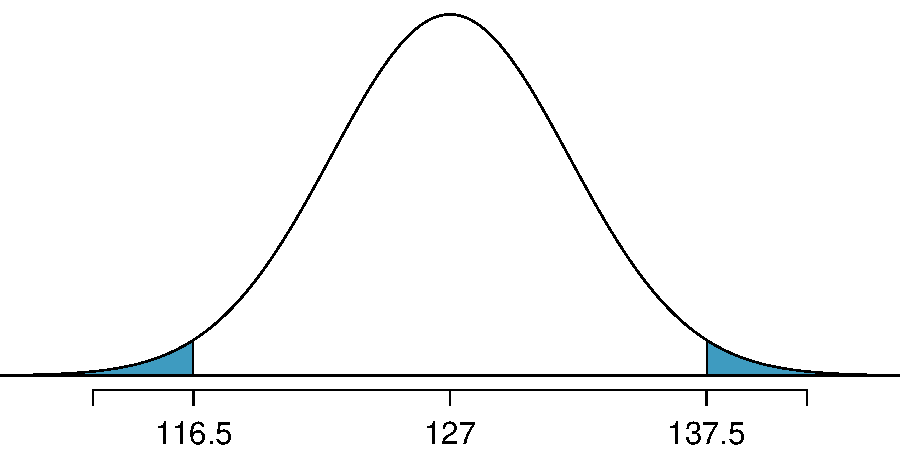
\includegraphics[width=\textwidth]{figures/04/ERwait} 
\end{center}
The data provide convincing evidence that the the average ER wait time has increased over the last year.
\end{minipage}
\item Yes, p-value $>$ 0.01, therefore we would fail to reject $H_0$ at $\alpha = 0.01$ and conclude that, at this significance level, the data do not provide convincing evidence to conclude that the average ER wait time has changed over the last year.
\end{parts}

\item[4.27]
\begin{parts}
\item $H_0$: Anti-depressants do not work for the treatment of Fibromyalgia. \\
$H_A$: Anti-depressants work for the treatment of Fibromyalgia. \\
Diana might also have taken special note if her symptoms got much worse, so a more scientific approach would have been to use a two-sided test. While parts (b)-(d) will rely on the one-sided version, your answers will be a little different if you used a two-sided test.
\item Concluding that anti-depressants work for the treatment of Fibromyalgia symptoms when they actually do not.
\item Concluding that anti-depressants do not work for the treatment of Fibromyalgia symptoms when they actually do.
\item If she makes a Type 1 error, she will continue taking medication that does not actually treat her disorder. If she makes a Type 2 error, she will stop taking medication that could treat her disorder.
\end{parts}

\item[4.41]
\begin{parts}
\item The distribution of the lengths of these songs is slightly right skewed to the right, therefore it is not reasonable to use a normal model to estimate this probability. However, we can approximate the probability using the histogram. It appears that there are 350 songs between whose lengths are between 5-6 mins, 100 songs between 6-7 mins, 25 songs between 7-8 mins, 20 songs between 8-9 mins and 5 songs between 9-10 mins. If we let X denote the length of a randomly chosen song, then,
\[ P(X > 5) = \frac{350 + 100 + 25 + 20 + 5}{3000} = \frac{500}{3000} = 0.17 \]
(Answers may vary a little.)
\item Two different answers are reasonable. 
\begin{enumerate}[(1)]
\item CLT conditions are met: \\
Since the population distribution is only slightly skewed to the right, even a small sample size may be sufficient to yield a nearly normal sampling distribution. We also know that the songs are sampled randomly and the sample size is less than 10\% of the population, therefore we can also assume that the length of one song in the sample is independent of another.  We are looking for the probability that the total length of 15 songs is more than 60 minutes. This means that one song on average should last at least $\frac{60}{15} = 4$ minutes.  
Then,
\begin{align*}
\bar{X} &\sim N \left( \mu_{\bar{x}} = 3.45, SE_{\bar{x}} = \frac{1.62}{\sqrt{15}}  \right)  \\
P(\bar{X} > 4) &= P \left( z > \frac{4 - 3.45}{\frac{1.62}{\sqrt{15}}} \right)= P(z > 1.31) = 1 - 0.9049 = 0.0951
\end{align*}
\item CLT conditions are not met: \\
Since the population distribution is not normal, a small sample size may not be sufficient to yield a nearly normal sampling distribution. Therefore, we cannot estimate the probability using the tools we have learned so far.
\end{enumerate}
\item We can now be confident that the conditions are satisfied (see part (b)). Therefore,

\begin{minipage}[c]{0.5\textwidth}
\begin{align*}
\bar{X} &\sim N\left(\mu_{\bar{x}} = 3.45, SE_{\bar{x}} = \frac{1.63}{\sqrt{100}}\right) \\
P(\bar{X} > 3.6 ) &= P\left(z > \frac{3.6 - 3.45}{\frac{1.63}{\sqrt{100}}}\right) \\
&= P(z > 0.92) \\
&= 1 - 0.8212 \\
&=  0.1788
\end{align*}
\end{minipage}
\begin{minipage}[c]{0.5\textwidth}
\begin{center}
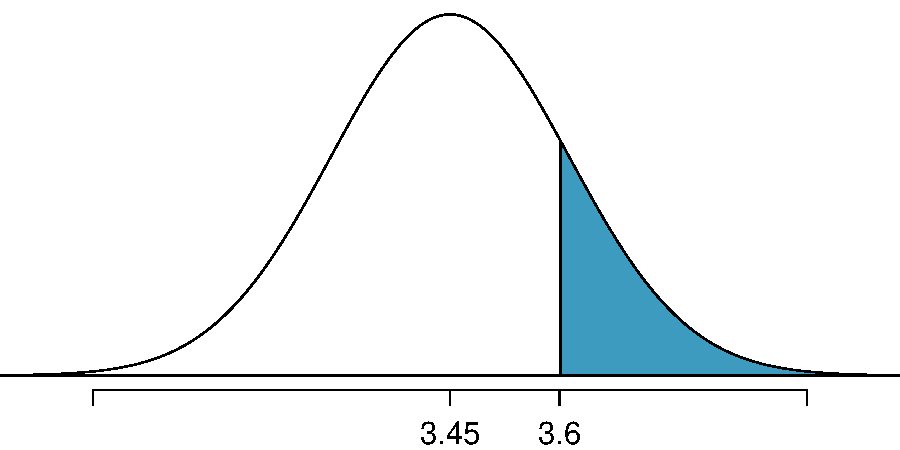
\includegraphics[width=\textwidth]{figures/04/ipod_n100.pdf}
\end{center}
\end{minipage}
\end{parts}

\item[4.43]
\begin{parts}
\item $H_0: \mu_{2009} = \mu_{2004}$: The average number of spam emails per day in 2009 is equal to the average in 2004. \\
 $H_A: \mu_{2009} \ne \mu_{2004}$:  The average number of spam emails per day in 2009 is different from the average in 2004.
\item The point estimate is $\bar{x}_{2009} - \bar{x}_{2004} = 14.9 - 18.5 = -3.6$ spam emails per day.
\item The null hypothesis is not rejected and these data do not provide convincing evidence that the true average number of spam emails per day in years 2004 and 2009 are different. The observed difference is about what we might expect from sampling variability alone.
\item Yes, the null hypothesis states that the population means are equal, and therefore the null value is 0. Since the null hypothesis is not rejected, we would expect the confidence interval to contain this value.
\end{parts}

\item[4.45]
\begin{parts}
\item $H_0: p_{2009} = p_{2004}$: The proportion of Americans who delete spam messages was the same in 2009 as it was in 2004. \\
 $H_A: p_{2009} \ne p_{2004}$: The proportion of Americans who delete spam messages was different in 2009 than it was in 2004.
 \item The point estimate is $\hat{p}_{2009} - \hat{p}_{2004} = 16 - 23 = -7\%$. The change over time is -7\%.
\item The null hypothesis is rejected and these data do provide convincing evidence that the true proportion of those who once a month or less frequently (or never) delete their spam email is higher in 2004 than in 2009. The difference is so large that it cannot easily be explained away as being due to chance.
\item No, the null hypothesis states that the population proportions are equal, and therefore the null value is 0. Since the null hypothesis is  rejected, we would not expect the confidence interval to contain this value.
\end{parts}

%\item[4.47]
%\begin{parts}
%\item Scenario I is higher. Recall that means from smaller samples tend to be less accurate and so have larger standard errors.
%\item Scenario I is higher. The higher confidence level, the higher the margin of error
%\item They are equal. The sample size doesn't affect the calculation of the p-value for a given Z score.
%\item Scenario I is higher. When significance level is higher the chance of falling to reject the null hypothesis is lower.
%\end{parts}
%
%\item[4.49]
%\[ 10 \ge 2.58 \times  \frac{102}{\sqrt{n}} \ \rightarrow \ n \ge \left( \frac{2.58 \times  102}{10} \right)^2 = 692.5319 \]
%He should survey at least 693 customers. Note that we need to round up the calculated sample size. 

\end{enumerate}






\end{document}